%%%%%%%%%%%%%%%%%%%%%%%%%%%%%%%%%%%%%%%%%%%%%%%%%%%%%%%%%%%%%%%%%%%%%%%%%%%%%%%%
\section{Design}
\label{sec:methodology}

The purpose of the S/P mode is to create a distinct separation between simple users and power users. This section details the design of the S/P mode toggle. Each Windows user account would offer the S/P mode toggle directly on the login screen. This toggle does not alter the existing permission management systems of Windows or Unix-based operating systems.

\autoref{fig:demo_image} presents a prototype of the proposed login screen UI incorporating the S/P mode toggle. The key modification compared to the standard Windows login screen is the addition of a new button located on the right side of the existing login options. This button allows users to directly select either S Mode or P Mode from the login interface. The system remembers the user’s previous choice: if S Mode was selected during the last session, it will default to S Mode; likewise, if P Mode was chosen, it will default to P Mode unless the user opts to switch. Notably, this enhancement is strictly a UI-level adjustment and does not alter the underlying functionality for user accounts, whether they are administrators, sudo users, or regular users. Instead, it introduces a secure and intuitive interface to complement the existing account structure without changing the way users interact with the system. When the user selects S Mode, the operating system does not launch the standard desktop UI. Instead, it uses Microsoft Edge as the engine for running PWAs and presents a UI similar to iPhone or Android, where users can access and launch PWAs in an intuitive, app-like interface. This design enhances accessibility while maintaining the simplicity of the PWA-focused environment.

\begin{figure}[t] % Use figure* for full-width images in two-column layouts
\centering
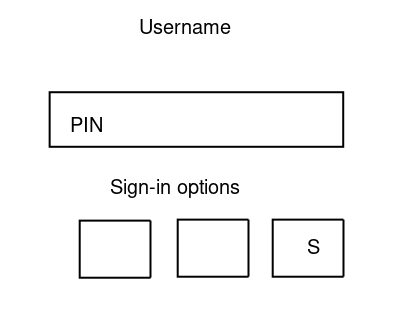
\includegraphics[width=0.4\textwidth]{demo.jpg} % Set to full text width
\caption{Demo of the S/P Mode Toggle Login Screen}
\label{fig:demo_image}
\end{figure}


\subsection{S Mode}

\autoref{fig:smodearch} illustrates the architecture diagram for the S Mode toggle, while \autoref{fig:walledgarden} depicts the scope of the PWA Walled Garden. S Mode is specifically designed for users who focus on essential tasks such as working with Word, Excel, or engaging with social media apps like YouTube and Instagram, supported through progressive web apps. Advanced functionalities intended for power users are omitted in this environment. The primary goal of S Mode is to implement stringent controls, with restrictions surpassing those enforced on iPhones in numerous settings.

\begin{figure}[h!]
\centering
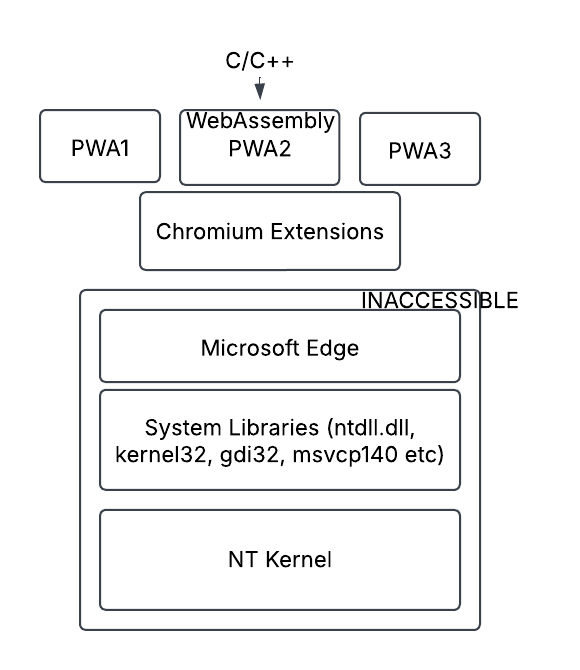
\includegraphics[width=0.4\textwidth]{smodearch.png}
\caption{S Mode Toggle Architecture (NOT Windows S mode)}
\label{fig:smodearch} % Label for referencing the image in the paper
\end{figure}

\begin{figure*}[h!]
    \centering
    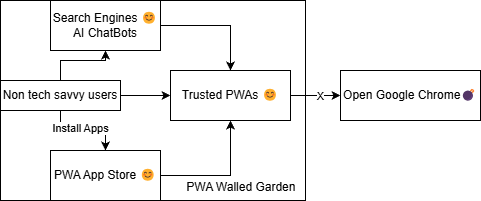
\includegraphics[width=0.6\linewidth]{walledgarden.png}
    \caption{PWA Walled Garden in S Mode Toggle (NOT Windows S mode)}
    \label{fig:walledgarden}
\end{figure*}

\subsubsection{Disallow Direct Browser Use}

Browsers are considered unsafe and are strictly prohibited for direct use. They are only permitted for hosting PWAs. No application, including Microsoft Edge or third-party browsers like Google Chrome and Firefox, should provide standalone browser functionalities.

\subsubsection{Disallow Direct Search Engine Use}

Search engines are also regarded as unsafe and are disallowed in S Mode. This restriction helps prevent phishing attempts, blocks access to fake websites, and mitigates the growing issue of SEO pollution\cite{10.1007/978-3-031-56063-7_4}. Users are limited to searching only within the websites of installed PWAs, and are encouraged to rely on AI-powered chatbots, such as Microsoft Copilot, ChatGPT, or Deepseek, for accessing web content securely.

\subsubsection{Browser Running Within the App Sandbox in S Mode}

In S Mode, the browser application itself should operate within the App Sandbox\cite{MicrosoftAppIsolationOverview} to add an additional layer of defense. This setup ensures that PWAs are not only sandboxed by the browser but also benefit from the security of the App Sandbox encapsulating the browser. This dual-layer protection strengthens security by combining the isolated environments of both the browser and the App Sandbox.

\subsubsection{All Progressive Web Apps Must Be Installed via the App Store}

Progressive web apps are installed in a manner similar to traditional apps on platforms like Google Play Store or Apple App Store. However, instead of native apps, users install PWAs. These apps run internally using Microsoft Edge, but direct access to the browser itself is restricted.

\subsubsection{Browser Extensions are in the App Store}

Since PWAs operate within browsers, they often leverage browser extensions. For example, users might install ad blockers for YouTube PWAs or use global speed/pitch adjusters to modify playback speeds for apps like Spotify, transforming them into nightcore players. To maintain control, such extensions should be made available only through the App Store.

\subsubsection{Restrict Direct URL Access}

Allowing users to type URLs poses risks, as typographical errors can lead to security issues. Hence, direct URL access is prohibited in all forms within S Mode.

\subsubsection{PWA App Store Must Be Open}

Progressive Web Apps are web resources and should remain open to ensure accessibility and transparency. Developers should have the ability to submit their PWAs to a publicly available GitHub repository, akin to how Microsoft vcpkg operates, or alternatively, rely on web standards to oversee PWA App Stores. Furthermore, no commission fees should be allowed for app submissions. This openness enables other operating systems, such as Linux and macOS, to adopt and implement this security model effectively.

\subsubsection{Limit External Links}

Web pages often include external links that could redirect users to malicious websites. To address this, PWAs must include a manifest file specifying a whitelist of allowed external links. By default, login pages for services like Google, Apple, or Microsoft accounts are permitted unless explicitly restricted by the app.

\subsubsection{Restrict Permission Changes}

Modern apps frequently request excessive permissions to exploit user data. In S Mode, users are prohibited from modifying app permissions to maintain data security.

\subsubsection{Disallow Sideloading}

Sideloading of both PWAs and browser extensions is strictly prohibited in S Mode.

\subsubsection{Restrict Basic Settings Changes}

Even seemingly simple settings, like date and time or timezone configurations, can be problematic for users. Incorrect settings often disrupt app functionality, such as the Google Play Store. To reduce complexity and maintenance needs, these settings cannot be altered in S Mode.

\subsubsection{Restrict File Access to \texttt{\$HOME/.smode} Directory}

Complete restriction of file access is impractical, yet unrestricted access poses significant risks, as demonstrated by historical issues with Windows Phone. In S Mode, file access is limited to the \texttt{\$HOME/.smode} directory (\%USERPROFILE\%/.smode on Windows), ensuring essential functionality while minimizing potential vulnerabilities. Additionally, users can synchronize their data seamlessly with Microsoft OneDrive within S Mode. However, apps should NEVER be allowed to access Microsoft OneDrive directly to prevent ransomware.

\subsubsection{App Transitions Restricted to Installed PWAs}

If one PWA attempts to open another PWA, the transition must be limited to installed PWAs. A browser popup should appear to handle the transition, but if the target PWA is not installed, the app transition should be blocked.

\subsubsection{Gradually Implement Enhanced Security Measures for PWAs}

Progressive Web Apps should gradually adopt stronger security measures to improve their robustness. For instance, WebAssembly binaries—often compiled from memory-unsafe languages like C/C++—require additional mitigations, such as WebAssembly Memory Tagging\cite{webassemblymemorytagging}, to ensure safer execution. S Mode offers an opportunity to enforce stricter security measures for PWAs. However, as most WebAssembly applications currently lack adequate mitigations, this process must be introduced incrementally to allow for widespread adoption and compatibility.

\subsubsection{S Mode UI Should Closely Resemble iPhone's UI}

The iPhone's UI has become the de facto standard for mobile phone interfaces and walled garden operating systems. As mobile UIs are the most familiar to a majority of end users, adopting a similar design for S Mode ensures ease of use and eliminates any learning curve for users. 

\subsubsection{Automatic PWA Synchronization}

Currently, PWAs are synchronized through Microsoft Edge, making them easily accessible for end users. To enhance usability in S Mode, these PWAs should be automatically synced, ensuring a seamless experience for users.

\subsubsection{Integration with Trusted Platform Module for Sensitive Apps}

Sensitive PWAs, such as the Chase Bank App, can enhance security by leveraging the Trusted Platform Module\cite{10.1145/3320269.3372197} to verify the integrity of both the Edge browser engine and the banking application's code. This ensures that sensitive operations are executed within the app's sandbox, with their integrity fully guaranteed.

\subsection{P Mode}

P Mode represents the Windows environment in its standard form. It allows users to perform tasks such as running \texttt{.exe} files, utilizing browsers, accessing the Windows Subsystem for Linux, using \texttt{cmd} and PowerShell, editing the registry (\texttt{regedit}), and rebooting into UEFI to install other operating systems. Logging into P Mode signifies that the user is a power user, comparable to utilizing \texttt{unsafe} blocks in programming languages like C\# or Rust. It conveys to the operating system: "I understand the risks and am fully capable of managing them. Please grant me unrestricted access to perform my tasks."

With the introduction of the S/P mode toggle, P Mode also takes on the responsibility of managing settings for S Mode. Below, we present the design principles for P Mode.

The Windows Settings app in P Mode should include a dedicated section for managing S Mode settings.

\subsubsection{Power User Mode Must Grant Full Control, Including Installation of Other Operating Systems}

P Mode is designed for power users and is not intended to be a locked-down environment. Power users should not face the restrictions common to ecosystems like Android or iOS. Instead, P Mode must allow users complete freedom, including the ability to install alternative operating systems.

\subsubsection{Enable Comprehensive Settings Management}

While S Mode restricts changes to date, time, and timezone settings, P Mode must provide full access to these configurations. This highlights the versatility of the S/P mode toggle compared to fully locked platforms like iPhones, where errors in settings can arise due to the absence of boundaries for unsafe operations. In the pursuit of complete safety, unintended vulnerabilities may emerge—this toggle offers a balance.

\subsubsection{Allow Sideloading of PWAs and Browser Extensions into S Mode}

Since PWAs are essentially websites, sideloading them into S Mode should be straightforward—users can simply input URLs to initiate the process. Additionally, the Edge browser in P Mode can feature an option that allows users to install PWAs and Chromium extensions directly into S Mode.

\subsubsection{Centralized Permission Management for PWAs in S Mode}

Permissions for PWAs in S Mode should be managed exclusively through P Mode. Android apps often manipulate users into granting unnecessary permissions. By centralizing permission management in P Mode, this approach protects non-tech-savvy users from being tricked by applications while retaining full functionality for power users.

\subsubsection{Adjust PWA Synchronization Settings}

P Mode should offer users the flexibility to customize how PWAs are synchronized for S Mode. This ensures personalized and efficient use of PWAs.

\subsubsection{Modify File Access Settings for S Mode}

By default, file access in S Mode is restricted to \texttt{\$HOME/.smode} (On Windows it is \texttt{\%USERPROFILE\%/.smode}) directory. In P Mode, users should be able to expand access by adding more directories or modifying the default directory that S Mode can access.

\subsubsection{Dedicated File Storage for Each PWA}

In addition to shared storage for Progressive Web Apps, each PWA can maintain its own dedicated file storage. This approach enhances sandboxing capabilities in S Mode, ensuring greater isolation and security for individual app.

\subsubsection{Popup Suggestions for Entering S Mode in Sensitive Apps}

Sensitive applications, such as banking PWAs like Chase, require heightened security measures. In this context, browsers operating in power user mode should provide a discreet suggestion prompting users to switch to S Mode for enhanced protection. To ensure a seamless user experience, these prompts should be limited in frequency and appear only for sensitive applications. Unless mandated by a bank's policy to enforce the use of S Mode, these suggestions should remain optional, allowing users to make the choice without feeling overwhelmed by intrusive notifications.

\subsubsection{Gradually Expand Options for Modifying S Mode Settings}

The aforementioned list outlines initial options for modifying S Mode settings. Over time, users may require additional flexibility, such as changing the browser engine used for PWAs instead of relying solely on Microsoft Edge. However, this introduces potential security risks—if the browser engine originates from a malicious source, it could compromise the entire system, as illustrated by scenarios like using a Chase Bank PWA. To mitigate these risks, modifications should only be allowed through the App Store in P Mode or by requiring cryptographic signatures provided by Microsoft to verify the integrity of the browser engine. These changes must be implemented with caution and gradually.

Additional options, such as enabling the sideloading of Win32 sandbox applications into S Mode, could pose significant security risks. Unfortunately, many apps vendors—such as WeChat—choose to monetize user data rather than offering PWAs. To ensure the security and integrity of S Mode, these features must be implemented thoughtfully and incrementally. Nonetheless, Progressive Web Apps should remain the preferred method for app delivery over Win32 sandbox applications, as PWAs inherently add an extra layer of sandboxing through the browser engine.
